
\documentclass[]{article}

%Packages
\usepackage[spanish]{babel}
\usepackage[utf8]{inputenc}
%Fórmulas
\usepackage{amsmath, amsthm, amssymb}
%Imágenes
\usepackage{graphicx}

%Keywords en español
\newenvironment{keywords}
{\par\noindent\small\textbf{\keywordsname:}}
{\par}
\addto\captionsspanish{\def\keywordsname{Palabras Claves}}






\begin{document}
\selectlanguage{spanish}

\title{Premios Nobel Medicina y Fisiología 2018 }

\author{Alicia Isabel Pérez Lorente}



\maketitle              


\begin{abstract} https://github.com/aliciapl/proyecto\_final \\
	En este trabajo se presenta a los dos galardonados con el Premio Nobel de Fisiología y Medicina de 2018. Los doctores galardonados con dicho premio han sido James P. Allison y Tasaku Honjo por su descubrimiento de la terapia contra el cáncer mediante la inhibición de la regulación inmune negativa.

\begin{keywords}
Cáncer, Inmunoterapia, Nobel, Allison, Honjo, PD1, CLTA4.
\end{keywords}


\end{abstract}


\section{Introducción}
El nobel en 2018 en la categoría de Fisiología y Medicina lo han recibido James P. Allison y Tasaku Honjo por su descubrimiento de la terapia contra el cáncer mediante la inhibición de la regulación inmune negativa. En sus experimentos, se aprovecha la capacidad del sistema inmune para atacar las células cancerosas al liberar los frenos de las células inmunitarias.

\begin{table}[!h]
	\centering
	\caption{Premios Nobel anteriores}
	\label{tab1}
	
	\begin{tabular}{c|c|c|}
		\cline{2-3}
		
		& \textbf{Galardonados} & \textbf{Descubrimiento} \\ \hline
		
		\multicolumn{1}{|c|}{\textbf{2017}} &   Rosbash and Hall                     &    Mecanismos moleculares que controlan el ritmo circadiano             \\ \hline
		\multicolumn{1}{|c|}{\textbf{2016}} &   Ohsumi                    &          Mecanismos de la autofagia             \\ \hline
		\multicolumn{1}{|c|}{\textbf{2015}} &     Omura and Youyou                 &          Nueva terapia contra la malaria             \\ \hline
		\multicolumn{1}{|c|}{\textbf{2014}} &         May-Britt Moser              &      Células del disposicionamiento en cerebro                 \\ \hline
	\end{tabular}%
	
\end{table}

\section{Estado del arte}
Desde 1962 se comenzaron estudios basados en la inmunoterapia contra tumores, demostrándose a partir de esos años la existencia de antígenos frente a tumores específicos y su naturaleza molecular.
En 1996, James P. Allison y colaboradores demostraron que los anticuerpos en contacto con la superficie de las células T, CTLA-4, son capaces de desencadenar una respuesta inmune, curando así tumores en ratones (ver Figura \ref{fi}). 
Previamente, Tasuku Honjo et al. \cite{Dong2003} identificó una nueva molécula, PD-1. De forma análoga a CTLA-4, PD-1 sirve también como freno, evitando que las células T ataquen a las células cancerosas. 
James P. Allison desarrolló el concepto de anti-CTLA-4 en el ámbito clínico con individuos con melanomas. 



\begin{figure}[!h]
	\centering
	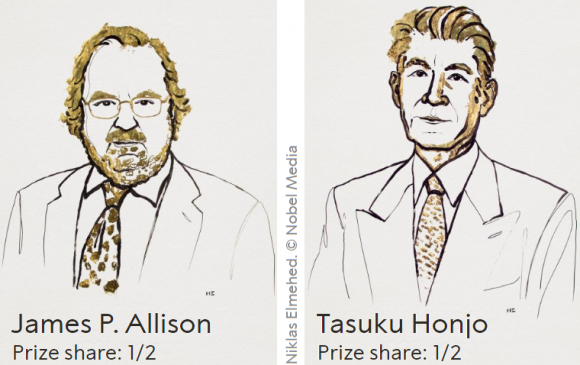
\includegraphics[width=0.8\textwidth]{images/caras.png}
	\caption{ Ganadores Premio Nobel 2018. } \label{fi}
\end{figure}

\section{Resultados y discusión}
Identificación de CTLA-4 como regulador negativo: Pertenece a la misma superfamilia de inmunoglobulinas que CD28. La inactivación del gen ctla4 en ratones confirmaron que la proteína CTLA-4 es un regulador negativo, puesto que tras la eliminación de dicho gen, los ratones desarrollaron graves enfermedades autoinmunes.
Inhibición del crecimiento de tumores usando anticuerpos contra CTLA-4 en animales: Allison dirigió su investigación a intentar bloquear los efectos negativos provocados por CTLA-4, desencadenando además una respuesta inmunitaria.Esto se recoge en el trabajo de Hansen et al. \cite{Hansen1980}  Como se observa en la gráfica, los experimentos confirmaron que bloqueando CTLA-4, se potencia la respuesta de las células T  contra tumores (ver Figura \ref{fi2}). 
Desarrollo de la terapia clínica de inhibición del checkpoint: Se consiguió desarrollar anticuerpos monoclonales IgG1 anti-CTLA-4, denominados MDX-010. En 2003, se hicieron ensayos clínicos en fase I con 9 pacientes, registrándose en algunos casos una regresión del melanoma, desarrollándose en algunos casos respuestas autoinmunes. Esto se recoge en el artículo de Takunsu el al. \cite{Tasuku} .  



\begin{figure}[!h]
	\centering
	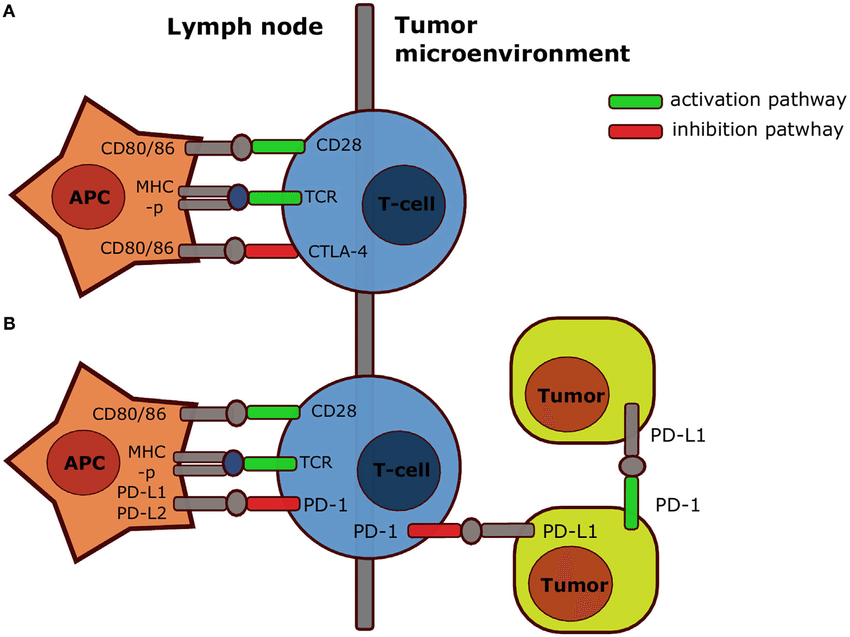
\includegraphics[width=0.8\textwidth]{images/PD1.png}
	\caption{ Role de CTLA-4 y PD-1 en tumores. } \label{fi2}
\end{figure}



\section{Fórmula}
La ecuación de Monod presentada (\ref{eq}) explica el crecimiento exponencial de una población o grupo de células.

\begin{equation} \label{eq}
dx/dt=\frac{mumax*S}{Ks+S-}*x
\end{equation}

\bibliographystyle{unsrt}
\bibliography{biblio}



\end{document}
